%\documentclass{article}
%\usepackage{pgfplots}
%
%\begin{document}
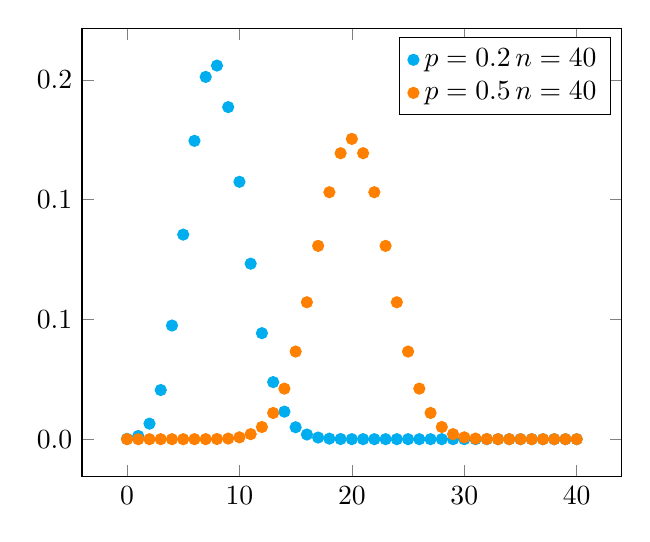
\begin{tikzpicture}[
    declare function={binom(\k,\n,\p)=\n!/(\k!*(\n-\k)!)*\p^\k*(1-\p)^(\n-\k);}
]
\begin{axis}[
    samples at={0,...,40},
    yticklabel style={
        /pgf/number format/fixed,
        /pgf/number format/fixed zerofill,
        /pgf/number format/precision=1
    }
]
\addplot [only marks, cyan] {binom(x,40,0.2)}; \addlegendentry{$p=0.2 \, n=40$}
\addplot [only marks, orange] {binom(x,40,0.5)}; \addlegendentry{$p=0.5 \, n=40 $}
\end{axis}
\end{tikzpicture}
%\end{document}